
The verification of execution relies on a concept called
zero-knowledge proof. A zero-knowledge proof is a cryptographic
protocol that can be used by one party, the prover, to prove to
another party that some statement is true without revealing additional
information.

//TODO skriv här

\begin{center}
  \makebox[\textwidth]{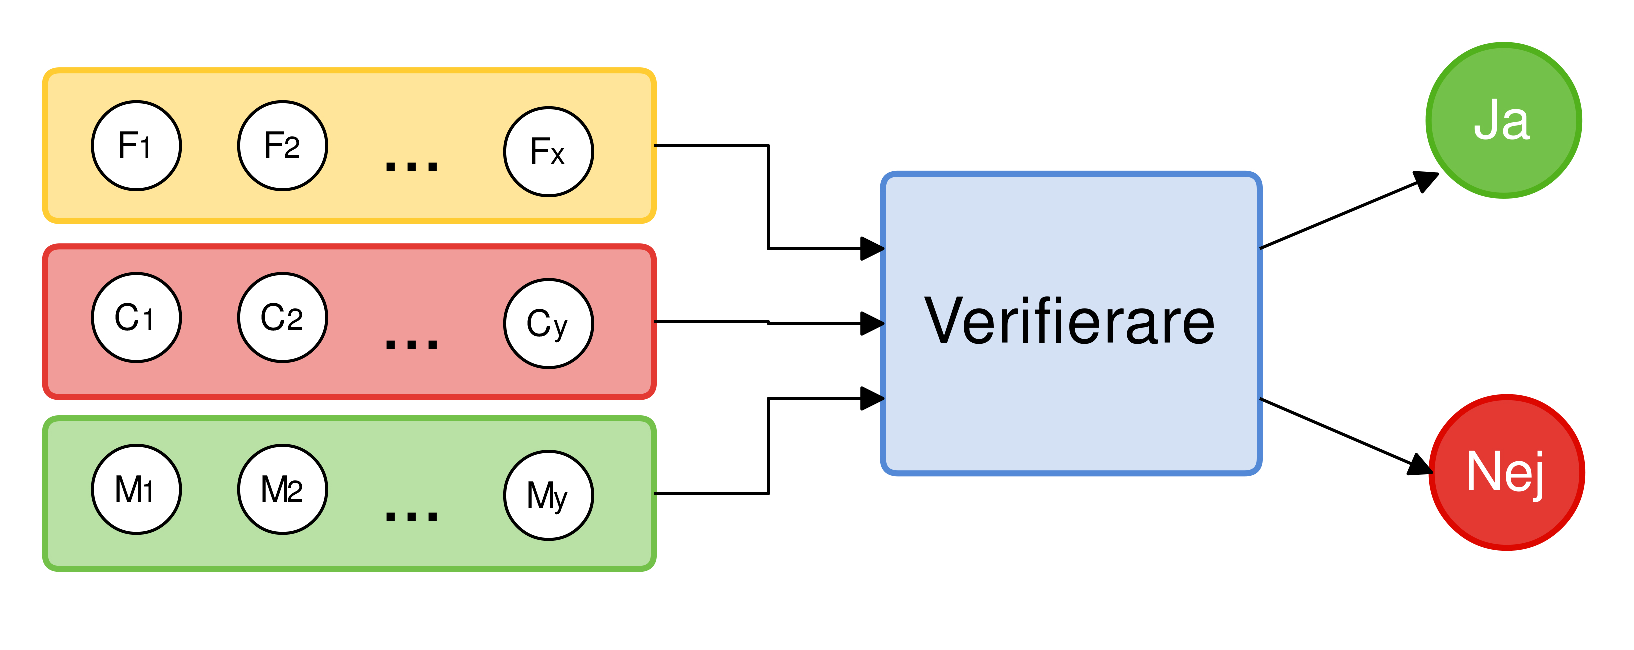
\includegraphics[width=\textwidth]{../presentation/images/mix3.pdf}}
\end{center}

